\documentclass[../main/main.tex]{subfiles}

\newdate{date}{25}{10}{2019}


\begin{document}


\chapter{Role of the models in statistical mechanics}
\marginpar{ \textbf{Lecture 6.} \\  \displaydate{date}. \\ Compiled:  \today.}
\section{Role of the models}
Which is the role of models in statistical mechanics? There are two possible approaches:
\begin{enumerate}
  \item The model must describe the real system in a very detailed way. The maximum number of details and parameters to be tuned are included. The \emph{pro} is the closer to the real specific system (faithfull description). The \emph{drawback} is that the model is so complicated that no analytical solution is possible. Moreover, even numerically, these models can be studied for very short times and small sizes.
  An example is the simulation of the folding dynamics that can be performed for few nanoseconds. On the other hand the introduction of many details are often not crucial if one is interested in large scale properties.
  \item Try to introduce the most simple model that satisfies few essential properties of the real system such as its symmetries, dimensionality, range of interactions etc.
  Since most of the microscopic details are integrated, these models cannot describe the full physics of a specific system but they can reproduce its main features. Moreover these models can be studied numerically and, to some extent also analitically (exact solution).
\end{enumerate}

It is the latter approach that we shall take here.
  Let us start by introducing what is, perhaps, the most paradigmatic model in the statistical mechanics of phase transition, the \emph{Ising model}.

  \section{The Ising model}
  Suggested by Lenz to Ising for his PHD thesis (1925), it is supposed to describe a magnetic system that undergoes a transition between a paramagnetic and a ferromagnetic phase.
  In \( d=1 \) the model was solved exactly by Ising. Unfortunately, he found that for \( T>0 \) the model does not display a phase transition.

  The wrong conclusion was that this model was not able to describe a phase transition. In fact, it turns out that, for \( d>1 \), the model does display a paramagnetic-ferromagnetic phase transition.

   Let us first discuss some general feature of the model for any dimension \( d \).

\subsection{\emph{d}-dimensional Ising model}
For hypercubic lattice with  given \( N(\Omega ) \) sites \( \{ i \}_{i=1,\dots,N(\Omega )}   \) and linear size \( L(\Omega ) \), we have
\begin{equation*}
   N (\Omega ) = L^d
\end{equation*}
 The microscopic degrees of freedom are the spins \( S_i \), defined at each \emph{i}-esim lattice site. Each spin can assume the values  \( S_i = \pm 1 \), that means that at each site the possible values are the spin up or down.
 For a lattice with \( N(\Omega ) \) spins, there are \( 2^{N(\Omega )} \)  possible configurations.
 \begin{remark}
 Since we do not consider the spin as a vector, this is a model for a strongly anysotropic ferromagnet (along a given direction).
 \end{remark}
 The minimal model that can try to capture the interaction between the spin is the following.
Suppose to have also an external magnetic field \( H_i \) (it values depends on the site \emph{i}). One can consider interactions between spins whose strength are described by functions \( J_{ij},k_{ijk}, \dots \). For instance, there is a coupling that derives from electrons coupling
\begin{equation*}
  J_{ij} = f ( \abs{\va{r_i}- \va{r_j}  } )
\end{equation*}
The physical origin is the overlap between the electronic orbitals of the neighbouring atoms forming the Bravais lattice.
Remember that a term as \( \sum_{i}^{} S_i  \) is not correlated, while we need an interaction for describing the model.

A general Hamiltonian of the model can be written as:
\begin{equation}
  \mathcal{H}_ \Omega ( \{ S_i \}  ) = \sum_{ij}^{} J_{ij} S_i S_j - \sum_{i}^{} H_i S_i - \sum_{ijk}^{} S_i S_j S_k + \dots
\end{equation}
Standard Ising model one keeps only the two-body interactions:
\begin{empheq}[box=\myyellowbox]{equation}
  \mathcal{H}_ \Omega ( \{ S_i \}  ) = -\frac{1}{2}\sum_{i\neq j}^{N} J_{ij} S_i S_j - \sum_{i=1}^{N} H_i S_i
\end{empheq}
where the first term represents a two body interaction that is a quadratic term, while the second term is a one body interaction.  We have put the minus because we want to minimize the energy, but it dipends on the sign of  \emph{J}.

For this model the sum over all configurations on trace is given by
\begin{equation}
  \Tr \equiv \sum_{S_1 = \pm }^{}  \sum_{S_2 = \pm }^{}  \dots \sum_{S_N = \pm }^{} \equiv \sum_{\{ S \}  }^{}
\end{equation}
 Our problem is to find the partition function with \emph{N} sites, which depends on \emph{T} and in principle depends in the configuration given (it is fixed both for \emph{H} and \emph{J}!).
Hence, the canonical partition function is given by
\begin{equation}
  Z_{\Omega } (T, \{ H_i \}, \{ J_{ij} \}    ) = \Tr e^{-\beta \mathcal{H}_ \Omega ( \{ S \}  )}
\end{equation}
and the corresponding \emph{free-energy},
\begin{equation}
  F_ \Omega  (T, \{ H_i \}, \{ J_{ij} \} ) = - k_B T \ln{Z_ \Omega }
\end{equation}
The \emph{bulk limiting free energy} is:
\begin{equation}
  f_b (T, \{ H_i \}, \{ J_{ij} \} ) = \lim_{N \rightarrow \infty }\frac{1}{N}  \ln { F_ \Omega  }
\end{equation}
How do we know that the above limit does exist? It must be proven. The surface is not important in the bulk limit.
 Note that we are assuming that the interaction between the spin is a short range force, it is not as the size of the system.

For this model it is possible to show that the limit exists if
\begin{equation}
  \sum_{j \neq i}^{} \abs{J_{ij}} < \infty
\end{equation}
\begin{remark}
In general what determines the existence of the limit of these spin models are the dimension \emph{d} and the range of the spins interactions.
\end{remark}
For example it is possible to show that, if
\begin{equation}
  J_{ij} = A \abs{\va{r_i}-\va{r_j}  }^{-\sigma}
\end{equation}
so it is a long range interaction, the limit exists when
\begin{equation*}
  \sigma > d
\end{equation*}
\begin{remark}
If the interaction is \emph{dipolar} since it decades as \( 1/r^3 \), for the case \( d=3 \) the limit does not exists. However, it is still possible to prove the existence of the limit for this case if one assumes that not all dipoles are fully aligned.
\end{remark}
Assuming that the thermodynamic limit exists, we now look at some additional rigorous results on the limiting free energy and its derivatives.

\subsection{Mathematical properties of the Ising model with neirest neighbours interactions}
For simplicity let us consider the case in which the external magnetic field is homogeneous, i.e. \( H_i \equiv H \), and the spin-spin interaction is only between spins that are nearest-neighbours (n.n.) on the lattice:
\begin{equation}
J_{ij} =
  \begin{cases}
  J & \text{if } i \text{ and } j \text{ are n.n.} \\
  0 & \text{otherwise}
  \end{cases}
\end{equation}
Now, the model is very simple:
\begin{equation}
  - \mathcal{H}_ \Omega ( \{ S \}  ) = J \sum_{\expval{ij} }^{N (\Omega )} S_i S_j + H \sum_{i}^{N(\Omega )} S_i
  \label{eq:6_0}
\end{equation}
where the notation \( \expval{ij}  \) means a double sum over \emph{i} and \emph{j}, with the constraint that \emph{i} and \emph{j} are nearest-neighbours.

Since \emph{H} is uniform, the average magnetization per spin is
\begin{equation}
  \expval{m} = \frac{1}{N (\Omega )} \sum_{i=1}^{N (\Omega )} \expval{S_i}
\end{equation}
where \( \expval{\dots}  \)  means average over the chosen ensemble.

\begin{remark}
For \( J=0 \), \eqref{eq:6_0}  is the hamiltonian of a paramagnet. The only influence ordering the spins is the field \( H \). They do not interact, there are no cooperative ffects and hence no phase transition.
\end{remark}

Since
\begin{equation}
  \sum_{i=1}^{N} \expval{S_i} = \frac{1}{Z} \Tr \qty[\sum_{i}^{} S_i  e^{-\beta \mathcal{H}_ \Omega (\{ S_i \}  )} ]  = \frac{1}{Z} \Tr \qty[\sum_{i}^{} S_i \exp (\beta  J \sum_{\expval{ij} }^{N(\Omega )} S_i S_j + \beta H \sum_{i}^{N(\Omega )} S_i  )  ]
\end{equation}
it is easy to show that:
\begin{equation}
  \expval{m} = - \frac{1}{N} \pdv{F_ \Omega }{H}
\end{equation}
where
\begin{equation}
  F_ \Omega (T,J,H) = - k_B T \ln{Z_N (T,J,H)}
\end{equation}

Let us now consider the properties of the limiting free-energy
\begin{equation}
  f_b = \lim_{N \rightarrow \infty } \frac{1}{N} (-k_B T \ln{Z_N} )
\end{equation}
\begin{greenbox}
  It is possible to prove the following properties:
  \begin{enumerate}
  \item \( f_b < 0 \).
  \item \( f_b (T,J,H) \) is a \emph{continuous} function of \emph{T,J} and \emph{H}.
  \item The right and left derivatives of \( f_b (T,J,H) \) exist and are equal almost everywhere.
  \item The molar entropy \( s = - \pdv{f_b}{T} \ge 0\)    almost everywhere.
  \item \( \pdv{f_b}{T}  \) is a \emph{monotonic non increasing} function of \emph{T}. That is \( \pdv[2]{f_b}{T} \le  0 \). This implies that:
  \begin{equation}
    c_H = T \qty(\pdv{S}{T} )_H = - T \qty(\pdv[2]{f_b}{T} )_H \ge 0
  \end{equation}
  \item \( \pdv{f_b}{H}  \) is a \emph{monotonic non increasing} function of \emph{H}. That is
  \begin{equation}
    \pdv[2]{f_b}{H} \le 0
  \end{equation}
  This implies that
  \begin{equation}
    \chi _T = \qty(\pdv{M}{H} )_T = - \qty(\pdv[2]{f_b}{H})_T \ge 0
  \end{equation}
  \end{enumerate}
\end{greenbox}
\begin{remark}
The above properties have been postulated in thermodynamics, but here they have been rigorously proved for the Ising model using statistical mechanics.
\end{remark}
\begin{proof} [Proof of property (4)]
  Almost everywhere we have to prove that:
  \begin{equation*}
    s \equiv - \pdv{f_b}{T} \ge 0
  \end{equation*}
  Let us consider a finite system
  \begin{equation}
  \begin{split}
  - \pdv{F_ \Omega }{T}   &= k_B \ln{(\Tr e^{- \beta \mathcal{H}_ \Omega }  )} + k_B T \frac{1}{k_B T^2} \frac{\Tr(\mathcal{H}_ \Omega  e^{-\beta \mathcal{H}_ \Omega } ) }{\Tr(e^{- \beta \mathcal{H}_ \Omega } ) } \\
  &= k_B \qty[\ln{Z} + \frac{\Tr(\beta \mathcal{H}_ \Omega e^{-\beta \mathcal{H}_ \Omega
  } ) }{Z_ \Omega } ] \underset{to\, do}{=}   - k_B T \Tr(\rho _ \Omega  \ln{\rho _ \Omega } )
  \end{split}
  \end{equation}
  where
  \begin{equation}
    \rho _ \Omega  = \frac{e^{-\beta \mathcal{H}_ \Omega } }{Z_ \Omega  }
  \end{equation}
  is the probability distribution.

  Since \( \rho _ \Omega \le 1 \) it implies \( \ln{\rho _ \Omega } \le 0  \) and so \( - \Tr(\rho _ \Omega ) \ln{\rho _ \Omega }   \) is positive. Then, let us divide by \( N (\Omega ) \) and take the thermodynamic limit:
  \begin{equation}
  \lim_{N \rightarrow \infty } - \frac{1}{N} \pdv{F_ \Omega }{T}   = - k_B T  \lim_{N \rightarrow \infty }  \frac{1}{N}  \underbrace{\Tr(\rho _ \Omega  \ln{\rho _ \Omega })}_{S _ \Omega }  = T s \ge 0  \quad \Rightarrow \quad s \ge 0
  \end{equation}
\end{proof}

All the other properties listed before (except \( (1) \)) are consequences of the \emph{convexity} property of \( f_b \).
\begin{orangebox}
  \begin{theorem}[]
  \( f_b  (T,J,H)\) is an upper convex (i.e. concave) function of \emph{H}.
  \end{theorem}
\end{orangebox}
\begin{proof}
The proof is based on the H$\ddot{o}$lder inequality for two sequences  \( \{ g_k \}, \{ h_k \}     \):
\begin{bluebox}
  \begin{definition}[H$\ddot{o}$lder inequality]
    Given  \( \{ g_k \}, \{ h_k \}     \) with \( g_k,h_k \ge 0, \forall k \) and two non negative real numbers \( \alpha _1, \alpha _2 \) such that \( \alpha _1 + \alpha _2 =1 \), the following inequality holds
    \begin{equation}
      \sum_{k}^{} (g_k)^{\alpha _1} (h_k)^{\alpha _2} \le \qty(\sum_{k}^{} g_k )^{\alpha _1} \qty(\sum_{k}^{} h_k )^{\alpha _2}
    \end{equation}
  \end{definition}
\end{bluebox}
Now, consider the partiction function:
\begin{equation}
  Z_ \Omega  (H) = \Tr[\exp (\beta H \sum_{i}^{} S_i ) \underbrace{\exp (\beta J \sum_{\expval{ij} }^{} S_i S_j ) }_{G (S)}  ] = \Tr [\exp (\beta H \sum_{i}^{} S_i ) G (S)]
\end{equation}
It implies that
\begin{equation}
  Z_ \Omega  (H_1 \alpha _1 + H_2 \alpha _2) = \Tr(\exp {\beta \alpha _1 H_1 \sum_{i}^{} S_i + \beta \alpha _2 H_2 \sum_{i}^{} S_i} G(S))
\end{equation}
On the other hand, since \( \alpha _1 + \alpha _2 =1 \):
\begin{equation}
  G (S) = G (S)^{\alpha _1} G(S)^{\alpha _2}
\end{equation}

\begin{equation}
    Z_ \Omega  (H_1 \alpha _1 + H_2 \alpha _2)   = \Tr[ (e^{\beta H_1 \sum_{i}^{} S_i } G (S))^{\alpha _1} (e^{\beta H_2 \sum_{i}^{} S_i } G (S))^{\alpha _2}]
\end{equation}
If we now apply the H$\ddot{o}$lder inequality we get
\begin{equation}
\begin{split}
    Z_ \Omega  (H_1 \alpha _1 + H_2 \alpha _2) & \le \qty(\Tr (e^{\beta H_1 \sum_{i}^{} S_i } G(S))^{\alpha _1}  ) \qty(\Tr (e^{\beta H_2 \sum_{i}^{} S_i } G (S))^{\alpha _2}  ) \\
    & = Z_ \Omega (H_1)^{\alpha _1} Z_ \Omega (H_2)^{\alpha _2}
\end{split}
\end{equation}
If we now take the logs and multiply by \( -k_B T \) both sides we have
\begin{equation}
  \lim_{N \rightarrow \infty } - \frac{1}{N} k_B T \ln{Z_ \Omega (H_1 \alpha _1 + H_2 \alpha _2)}  \ge
   - \lim_{N \rightarrow \infty } \frac{\alpha _1}{N} k_B T \ln{Z_ \Omega  (H_1 )} -
    \lim_{N \rightarrow \infty } \frac{\alpha _2}{N} k_B T \ln{Z_ \Omega  (H_2 )}  \\
\end{equation}
It implies
\begin{equation}
  f_b (H_1 \alpha _1 + H_2 \alpha _2) \ge \alpha _1 f_b (H_1 ) +  \alpha _2 f_b (H_2)
\end{equation}
That is a concave function of \emph{H}.
\end{proof}
\subsection{Ising model and \( \mathbb{Z}^2 \) symmetry. }
The symmetry of the system in sense of the Hamiltonian is: we can invert the value of the \emph{S} and the Hamiltonian does not change. It is valid when \( H=0 \), otherwise is not true. Let us see the \( \mathbb{Z}^2 \) symmetry and the following interesting relation:
\begin{orangebox}
  \begin{lemma}[]
  \( \forall  \) function \( \Phi  \) of the configuration \( \{ S_i \}   \), the following relation holds:
  \begin{equation}
    \sum_{ \{S_i = \pm 1\}}^{}  \Phi  (\{S_i\} ) =   \sum_{ \{S_i = \pm 1\}}^{}  \Phi  (\{-S_i\} )
      \label{eq:6_1}
  \end{equation}
  this is true for all function of the spin.
  \end{lemma}
\end{orangebox}
Now, we consider the hamiltonian of the Ising model:
\begin{equation*}
  - \mathcal{H}_ \Omega  = J \sum_{\expval{ij} }^{N(\Omega )} S_i S_j + H \sum_{i}^{N(\Omega )} S_i
\end{equation*}
Clearly,
\begin{equation}
  \mathcal{H}(H,J, \{S_i\}) =   \mathcal{H}_ \Omega (-H,J, \{-S_i\})
  \label{eq:6_1_1}
\end{equation}
This is a spontaneous broken symmetry.

Hence,
\begin{equation}
  \begin{split}
Z_ \Omega  (-H,J,T) &= \sum_{ \{S_i = \pm 1 \}}^{} \exp [-\beta \mathcal{H}_ \Omega  (-H,J, \{S_i\})]  \underset{\eqref{eq:6_1}}{=}   \sum_{ \{S_i = \pm 1 \}}^{} \exp [-\beta \mathcal{H}_ \Omega  (-H,J,\{-S_i\})] \\
&\underset{\eqref{eq:6_1_1}}{=} \sum_{ \{S_i= \pm 1\}}^{} \exp [-\beta \mathcal{H}_ \Omega  (H,J, \{S_i\}) ] = Z_ \Omega (H,J,T)
\end{split}
\end{equation}
Taking \( -k_B T \log  \)  and the \( \lim_{N \rightarrow \infty } \frac{1}{N} \)  we got:
\begin{equation}
  F_ \Omega  (T,J,H) = F_ \Omega  (T,J,-H)
  \label{eq:6_2}
\end{equation}
If we take the thermodynamic limit, we have
\begin{equation}
\Rightarrow f_b (T,J,H) = f_b (T,J,-H)
\end{equation}
and it means that the free energy density is an even function of \emph{H}!
\begin{remark}
From the finite-size relation \eqref{eq:6_2}, one can show that a \emph{finite-size}  Ising model does not display a transition to a ferromagnetic phase (for all dimension \emph{d}). Indeed,
\begin{equation}
    N (\Omega ) M(H) = - \pdv{F (H)}{H} \underset{\eqref{eq:6_2}}{=}  - \pdv{F(-H)}{(H)} = \pdv{F(-H)}{(-H)}  = - N (\Omega ) M (-H)
\end{equation}
Therefore:
\begin{equation}
  M (H) = - M (-H), \quad \forall H
\end{equation}
If \( H=0 \), we have \( M (0) = -M (0) \), that is valid if and only if \( M(0)= 0 \)!

The magnetization of a finite system is, at \( H=0 \), always zero. This is simply consequence of the symmetry argument shown above. It is only in the thermodynamic limit, where the symmetry is spontaneously broken.
\end{remark}

\section{Lattice gas model}
Even if we had not seen any transition, the Ising model is interesting because we can use this model to solve other problems that seems different but are not. In fact, the importance of the Ising model relies also on the fact that it can be mapped into other discrete systems. Despite its simplicity the Ising model is widely applicable because it describes any interacting two-state system. One of these applications is the \emph{lattice gas model}, where a gas is put in a lattice.

 What is a lattice gas model in more details?
 The archetypal lattice gas is a model where each lattice site can either be occupied by an atom or vacant.
 Let us consider a \emph{d}-dimensional lattice with coordination number \emph{z} and lattice spacing \emph{a}, divided into cell as in Figure \ref{fig:6_1} . Let us suppose that each cell is either empty or occupied by a single particle (this is more true if \( a \sim \SI{}{\angstrom}  \)).

 \begin{figure}[h!]
 \centering
 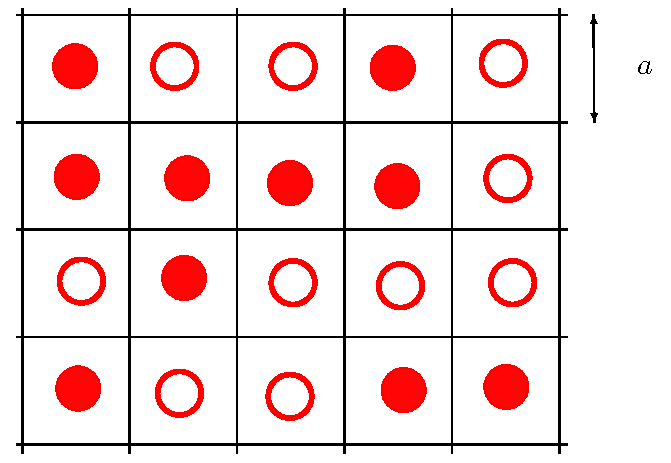
\includegraphics[width=0.6\textwidth]{../lessons/6_image/1.pdf}
 \caption{\label{fig:6_1} \( d \)-dimensional lattice with lattice spacing \( a \).}
 \end{figure}

 \noindent The \( n_i \) is the occupation of the \emph{i}-esim cell and it is:
\begin{equation}
n_i =
  \begin{cases}
   0 & \text{if empty} \\
   1 & \text{if occupied}
  \end{cases}
\end{equation}
We have:
\begin{equation}
  N _ \Omega = \sum_{i=1}^{N_c} n_i
\end{equation}
where \( N_c \) is the number of the lattice cells. In particular, \( N_c > N_{\Omega } \).

The hamiltonian of the model is
\begin{equation}
  \mathcal{H}_ \Omega  = \sum_{i=1}^{N_c} U_1 (i) n_i + \frac{1}{2} \sum_{ij}^{} U_2 (i,j) n_i n_j + O (n_i n_j n_k)
\end{equation}
where \( U_1 \) is for instance an external field, while \( U_2 \) is a many body interaction.

Since we want to work in the gran-canonical ensemble,
\begin{equation}
  \mathcal{H}_ \Omega  - \mu N_ \Omega  = \sum_{i=1}^{N_c} ( \cancel{ U_1 (i)} - \mu) n_i + \frac{1}{2} \sum_{ij}^{} U_2 (i,j) n_i n_j +   \dots
\end{equation}
and we put \( U_1=0 \) for convenience.

A formal relation with the Ising model can be obtained by choosing
\begin{equation}
  n_i = \frac{1}{2} (1+S_i) \quad \text{with } S_i = \pm 1
\end{equation}
The one body term becames:
\begin{equation}
  \sum_{i}^{} (U_1 (i) - \mu )  \frac{1}{2} (1+S_i) = \frac{1}{2} \sum_{i}^{} (U_1 (i) - \mu ) + \frac{1}{2} \sum_{i}^{} S_i (U_1 (i) - \mu )
\end{equation}
while the two bodies term is equal to:
\begin{equation}
  \frac{1}{2} \sum_{ij}^{} U_2 (i,j) \qty[\frac{1}{4} (1+S_i)(1+S_j)] = \frac{1}{8} 2 \sum_{ij}^{N_c} U_2 (i,j) S_i + \frac{1}{8}  \sum_{ij}^{N_c} U_2 (i,j) S_i S_j + \frac{1}{8} \sum_{ij}^{N_c} U_2 (i,j)
\end{equation}

Let us consider only short-range interactions, i.e.
\begin{equation}
U_2 (i,j) =
  \begin{cases}
   U_2 & i,j \text{ are n.n.}\\
   0 & \text{otherwise}
  \end{cases}
\end{equation}
It implies
\begin{equation}
    \frac{1}{2} \sum_{ij}^{} U_2 (i,j) \qty[\frac{1}{4} (1+S_i)(1+S_j)] =
      \frac{1}{4} z U_2 \sum_{i}^{N_c} S_i + \frac{U_2}{4} \sum_{\expval{ij} }^{} S_i S_j + \frac{1}{8} U_2 z N_c
\end{equation}
Remember that we put \( U_1 = 0 \) for simplicity:
\begin{equation}
    \mathcal{H}_ \Omega  - \mu N_ \Omega   =  E_0 - H \sum_{i=1}^{N_c} S_i - J \sum_{\expval{ij} }^{} S_i S_j
\end{equation}
where
\begin{subequations}
\begin{align}
     E_0 & = - \frac{1}{2} \mu N_c + \frac{z}{8} U_2 N_c \\
       -H &= - \frac{1}{2} \mu + \frac{z}{4} U_2 \\
         -J & = \frac{U_2}{4}
\end{align}
\end{subequations}
and remember that \emph{z} is the coordination number of neighbours.
 \( J \) is a nearest neighbour interaction which favours neighbouring sites being occupied.

The last equation implies:
\begin{equation}
  Z_{LG} = \Tr_{\{n\}}(e^{-\beta (\mathcal{H}_ \Omega -\mu N)} ) = e^{-\beta E_0} Z_{\text{Ising}} (H,J,N_c)
\end{equation}
We have seen that the Ising model is something more general than the magnetization transition.
In the next section, we show how to pass from the partition \( Z \) of a fluid, in the continuum, to the  \( Z_{LG} \) of the lattice gas model.

\section{Fluid system in a region \( \Omega  \) }
We can consider the system with periodic boundary condition, or within a box, or confined by an external one-body potential.

The hamiltonian for \emph{N} particles in \emph{d}-dimension is
\begin{equation}
  \mathcal{H}_ \Omega = \sum_{i=1}^{N} \qty[\frac{p_i^2}{2m} + U_1 (\va{r_i})] + \frac{1}{2} \sum_{i \neq j}^{} U_2 (\va{r_i}, \va{r_j}) + \frac{1}{3!} \sum_{i \neq j \neq k }^{}  U_3 (\va{r_i}, \va{r_j}, \va{r_k})
\end{equation}
In the gran-canonical ensemble we have:
\begin{equation}
  Z_ \Omega = \Tr(e^{-\beta (\mathcal{H}_ \Omega  - \mu N)} ) = \sum_{N=0}^{\infty } \frac{1}{N!} \int_{}^{} \prod_{i=1}^{N} \frac{\dd[d]{\va{p_i}} \dd[d]{\va{r_i}} }{h^{dN}} \qty(e^{-\beta (\mathcal{H}_ \Omega  - \mu N)} )
\end{equation}
and the gran-canonical potential is
\begin{equation}
  \omega _ \Omega (T, \mu , U_1, U_2, \dots) = -k_B T \ln{Z_ \Omega }
\end{equation}
\begin{remark}
\( \omega _ \Omega (\dots) \) even if it contains an infinite sum is not singular if \( \Omega  \) is finite!
\end{remark}
Indeed, if \( U_2 \) is an hard-core repulsion, each particle has a finite volume and, within a finite \( \Omega  \), only \( N_{max} \) particles can fit in
\begin{equation*}
  \Rightarrow \sum_{N=0}^{\infty } \sim \sum_{N=0}^{N_{max}}
\end{equation*}
In the thermodynamic limit it corresponds to
\begin{equation}
  \omega _ b (T, \mu , U_1, U_2, \dots) = \lim_{V (\Omega ) \rightarrow \infty } \frac{\omega
  _ \Omega }{V (\Omega )}
\end{equation}
with the contraint
\begin{equation*}
  \rho = \lim_{V \rightarrow \infty } \frac{\expval{N} }{V (\Omega ) } = const
\end{equation*}

Remember also that
\begin{redbox}
  \begin{equation}
  \dd[]{\omega _b (T, \mu )} = - \sigma \dd[]{T} - \rho  \dd[]{\mu } = - P
  \end{equation}
\end{redbox}
Now:
\begin{equation}
  Z_N = \sum_{N=0}^{\infty } \frac{1}{N!} \qty[\prod_{i=1}^{N}  \qty{ \int_{-\infty }^{+ \infty } \dd[d]{\va{p}} \frac{1}{h^{dN}} e^{-\beta \va{p_i}^2/2m}  } Q_N (T) ]
\end{equation}
On the other hand since \( \int_{}^{} \dd[]{x} e^{- \alpha x^2} = \sqrt{2 \pi / \alpha }    \),
\begin{equation}
  \int_{-\infty }^{+ \infty } \dd[d]{\va{p}} \frac{1}{h^{dN}} e^{-\beta \va{p_i}^2/2m} = \frac{1}{\Lambda (T)^d}
\end{equation}
where
\begin{equation}
  \Lambda ( T) = \frac{h}{\sqrt{2 \pi m k_B} T}
\end{equation}
Therefore,
\begin{equation}
  Z_ \Omega = \sum_{N=0}^{\infty } \frac{1}{N!} \qty(\frac{e^{\beta \mu } }{\Lambda (T)^d})^N Q_N
\end{equation}
with
\begin{equation}
  Q_N (T) = \int_{}^{} \prod_{i=1}^{N}  \dd[]{\va{r_i}}  e^{-\beta (U(\va{r}))}
\end{equation}


\subsection{From the continuous to the lattice gas model}
Let us divied \( \Omega  \) in discrete cells of size \emph{a}. If \emph{a} is approximate a repulsive range between particles we have that the probability that there is more than a particles sits in a cell is \( \ll 1 \). The potentials of the continuoum model depend on  \( \{ \va{r_i} \}   \).

Consider \( n_ \alpha = n_ \alpha (\va{r_i}) \) the occupation numbers. We have:
\begin{equation}
  \sum_{\alpha }^{} n_ \alpha = N = \int_{}^{} \dd[d]{\va{r}} \sum_{i=1}^{N} \delta (\va{r_i}-\va{r})= \int_{}^{} \dd[]{\va{r}} \rho (\va{r})
\end{equation}
where
\begin{equation}
  \rho (\va{r}) = \sum_{i=1}^{N}  \delta (\va{r_i}-\va{r})
\end{equation}
Moreover,
\begin{equation}
  \sum_{i}^{} U_1 (\va{r_i}) = \sum_{i}^{} \int_{\Omega }^{} \dd[d]{\va{r}} U_1 (\va{r})   \delta (\va{r_i}-\va{r}) = \int_{\Omega }^{} \dd[]{\va{r}}      U_1 (\va{r}) \rho (\va{r})
\end{equation}
We have \( U (\{ \va{r_i} \}  ) \rightarrow U (\{ n_ \alpha  \}  ) \) :
\begin{equation}
  Q_N \propto \int_{}^{} \prod_{i=1}^{N}  \dd[d]{\va{r_i}}   \rightarrow \sum_{\{ n_ \alpha  \} }^{}
\end{equation}
Indeed, for each configuration specified by the set \( \{ n_ \alpha  \}  \) there are \( N! \) possible configurations of \( \{ \va{r_i} \}  \). This is because the particles can exchange position between occupied cells.
Hence,
\begin{equation}
 Q_N \propto \int_{}^{} \prod_{i=1}^{N}  \dd[d]{\va{r_i}} \simeq N! (a^d)^{N_c} \sum_{\{ n_ \alpha = 0, 1 \}}^{'} \dots
\end{equation}
\begin{remark}
The symbol \( \sum_{}^{'}   \) means that the sum has the contraint that the toal number of particles is fixed to \emph{N}.
\end{remark}
Therefore,
\begin{equation}
  Q_N \propto N! (a^d)^N \sum_{\{ n_ \alpha  \} }^{'} e^{-\beta U ( \{ n_ \alpha  \} )}
\end{equation}
and
\begin{equation}
  Z_ \Omega  = \sum_{N=0}^{\infty } \frac{1}{N!} \qty(\frac{e^{\beta \mu } }{\Lambda ^d (T)}) ^N Q_N = \sum_{N=0}^{\infty } \qty[\qty(e^{\beta \mu} \frac{a}{\Lambda (T)}  )^d ]  ^N \sum_{\{ n_ \alpha  \} }^{'} e^{-\beta U ( \{ n_ \alpha  \} )}
\end{equation}
where \( \sum_{}^{'} = \sum_{\{ n_ \alpha  \} }^{}     \)  with the contraint \( \sum_{\alpha }^{} n_ \alpha = N   \).
\begin{remark}
In general it is difficult to perform sum with contraints. Fortunately, we are considering the gran-canonical ensemble.
Indeed, we can write
\begin{equation}
  \sum_{N=0}^{\infty} \sum_{\{ n_ \alpha  \}}^{'} f(n_ \alpha ) =   \underset{\sum_{\alpha }^{} n_ \alpha =0 }{\sum_{\{ n_ \alpha  \} }^{'}} f (n_ \alpha )  +
  \underset{\sum_{\alpha }^{} n_ \alpha =1 }{\sum_{\{ n_ \alpha  \} }^{'}} f (n_ \alpha )
  \dots +
    \underset{\sum_{\alpha }^{} n_ \alpha = \infty }{\sum_{\{ n_ \alpha  \} }^{'}} f (n_ \alpha ) =  \sum_{\{ n_ \alpha  \}} f(n_ \alpha )
\end{equation}
with no restriction.
\end{remark}
\begin{remark}
In the final sum all the \( 2^N \) possible microscopic states are inclued (considering \( U_1 =0 \)):
\begin{equation}
  Z_ \Omega ^{GC} \propto  \sum_{\{ n_ \alpha  \}} \exp [-\beta \qty(-\mu - \frac{D}{\beta } \log{\frac{a}{\Lambda }} ) \sum_{\alpha =0}^{N_c} n_ \alpha  + \beta U_2 \sum_{\expval{\alpha \beta } }^{} n_ \alpha n_ \beta + \dots     ]
\end{equation}
\begin{equation}
  \Rightarrow Z_ \Omega = \Tr e^{-\beta ( \mathcal{H}_ \Omega - \widetilde{\mu} N )} = Z_{LG} ( \widetilde{\mu } )
\end{equation}
where
\begin{equation}
  \widetilde{\mu } = \mu _{LG} = \mu _{phys} + D k_B T \log{\frac{a}{\Lambda }}
\end{equation}
\end{remark}
%%%%%%%%%%%%%




\chapter{Some exactly solvable models of phase transitions}

The bibliography of the entire chapter is taken by \cite{9_lesson_1},\cite{9_lesson_2},\cite{9_lesson_3}.


\section{\emph{1-dimensional} Ising model}
In this section, we arrive at the exact solution of the one dimensional Ising model.
 There are two techniques for solving the model:
\begin{enumerate}
\item the \emph{recursive method};
\item the \emph{transfer matrix method}.
\end{enumerate}

\subsection{Recursive method}

\subsubsection{Case with \( H=0 \) and free boundary conditions}

\begin{figure}[h!]
\centering
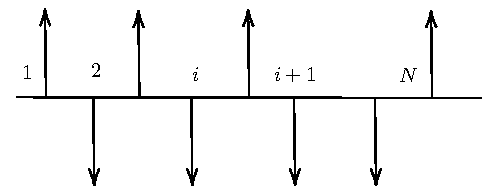
\includegraphics[width=0.5\textwidth]{../lessons/6_image/2.pdf}
\caption{\label{fig:6_2} One dimensional Bravais Lattice.}
\end{figure}

Consider a Bravais lattice in the one dimensional case, that is just a one dimensional lattice, as in Figure \ref{fig:6_2}.

The canonical partition function of such a system is:

\begin{equation}
  Z_N (T) = \sum_{S_1 = \pm 1}^{} \sum_{S_2 = \pm 1}^{} \dots  \sum_{S_N = \pm 1}^{} \exp [
  \overbrace{ \beta J}^{K}  \sum_{i=1}^{N-1} S_i S_{i+1}  ]
\end{equation}
The two body interaction is the sum in all the neighbours that in that case are \( (i-1) \)  and \( (i+1) \), but you have only to consider the one after, because the one behind is yet taken by the behind site.

Solve now this partition function. If we consider \emph{free boundary} condition, the \emph{N} does not have a \emph{N+1}, almost for the moment.
Let us define
\begin{equation}
   K \equiv \beta J,  \quad h \equiv \beta H
\end{equation}
Making explicit the sum in the exponential:
\begin{equation}
  Z_{N} (K) =   \sum_{S_1 = \pm 1}^{} \sum_{S_2 = \pm 1}^{} \dots  \sum_{S_N = \pm 1}^{} e^{K (S_1 S_2 + S_2 S_3 + \dots + S_{N-1}S_N)}
\end{equation}
What if we just add another spin at the end \( S_{N+1} \) ? Which is the partition function with that new spin? We obtain:
\begin{equation}
  Z_{N+1} (K) =   \sum_{S_{N+1} = \pm 1}^{} \sum_{S_1 = \pm 1}^{} \sum_{S_2 = \pm 1}^{} \dots  \sum_{S_N = \pm 1}^{} e^{K (S_1 S_2 + S_2 S_3 + \dots + S_{N-1}S_N)} e^{K S_N S_{N+1}}
\end{equation}
On the other hand, this sum is just involve this term:
\begin{equation}
   \sum_{S_{N+1} = \pm 1}^{} e^{K S_N S_{N+1}}  = e^{K S_N} + e^{-K S_N} = 2 \cosh (K S_N) = 2 \cosh(K)
\end{equation}
where the last equivalence derive from the fact that \( \cosh \) is an even function and it does not depend on \( \pm 1 \). Therefore:
\begin{equation}
  Z_{N+1} (K) = (2 \cosh (K) ) Z_N (K) \quad \text{and} \quad   Z_{N} (K) = (2 \cosh (K)) Z_{N-1} (K)
\end{equation}
By performing a backward iteration
\begin{equation}
  Z_N (K) = Z_1 (2 \cos(K) )^{N-1}
\end{equation}
Since \( Z_1 = \sum_{S_1=\pm1}^{} 1 = 2 \),
we have
\begin{empheq}[box=\myyellowbox]{equation}
   Z_N (T) = 2 (2 \cos(K) )^{N-1}
\end{empheq}
The free energy is:
\begin{equation}
  F_N (K) = - k_B T \ln{Z_N (K)} = - k_B T \ln{2} - k_B T (N-1) \ln{\qty(2 \cosh (K))}
\end{equation}
taking the thermodynamic limit it becames
\begin{equation}
  f_b (T) \equiv \lim_{N \rightarrow \infty } \frac{1}{N} F_N (K)= -k_B T \ln{\qty( 2 \cosh (\frac{J}{k_B T}))}
\end{equation}
As one can see \( f_b (T)  \) is an analytic function of \emph{T}, so we have no phase transition  at \( T \neq 0 \).

\begin{figure}[h!]
\centering
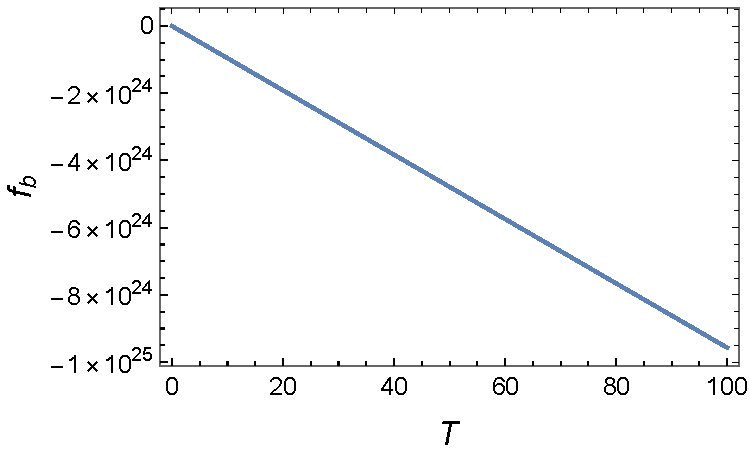
\includegraphics[width=0.45\textwidth]{../lessons/6_image/3.pdf}
\caption{\label{fig:6_3} Free energy function in thermodynamic limit for the one dimension Ising model.}
\end{figure}
We can compute the magnetization (the average over the spin \( \expval{S_j}  \)) for a generic site \emph{j}. This can be done in many ways. Assume again that \( S_i = \pm 1 \). Here, we choose one that consider another way to compute \emph{Z} for the \( 1-dimensional \) Ising model. This method can be useful for other calculations. It is based on the following identity:
\begin{equation}
  \exp [ K S_i S_{i+1}] \underset{to\,do}{=}  \cosh ( K) + S_i S_{i+1} \sinh (K) = \cosh (K) [1+ S_i S_{i+1} \tanh (K)]
\end{equation}
It means that
\begin{equation}
  Z_N (K) = \sum_{\{ S \}  }^{}    \exp [K  \sum_{i=1}^{N-1} S_i S_{i+1}  ] = \sum_{\{ S \}  }^{}   \prod_{i=1}^{N-1} [ \cosh (K) (1+ S_i S_{i+1} \tanh (K))]
\end{equation}
by rearranging,
\begin{equation}
  Z_N (K)= (\cosh K)^{N-1} \sum_{\{S\}}^{}  \prod_{i=1}^{N-1} ( 1 + S_i S_{i+1} \tanh K )
\end{equation}
If we now expand the products, we get terms of the following form:
\begin{equation}
  \sum_{ \substack{ S_{i_e} = \pm 1\\ e= 1, \dots, M} }^{}  (\tanh K )^M S_{i_1} S_{i_{1+1}} S_{i_2} S_{i_{2+1}} \dots S_{i_M} S_{i_{M+1}} = 0
  \label{eq:6_3}
\end{equation}
where \( i_1 \dots i_m \) is a set of \emph{M} sites of the lattice.
\begin{remark}
The terms above, when summed over \( \{ S \}   \) are zero, except the term with \( M=0 \) that is equal to 1 and, when summed over \( \{ S \}   \), gives \( 2^N \).
\end{remark}
Therefore:
\begin{equation}
  Z_N (K) = 2^N (\cosh K)^{N-1}
\end{equation}
that coincides with the result obtained before.

 If we now compute the average \( \expval{S_j}  \), the procedure is similar but now there will be terms as \eqref{eq:6_3} but with the addiction of an \( S_j \):
\begin{equation}
  (\tanh K)^M S_{i_1} S_{i_{1+1}} S_{i_2} S_{i_{2+1}} \dots S_{i_M} S_{i_{M+1}} \mathcolorbox{green!10}{S_j}
\end{equation}
that, when one sums over \( \{ S \}   \) are all zero, included the term with \( H=0 \) that now is equal to \( S_j \) and \( \sum_{S_j = \pm 1}^{} = 0   \). Hence, we have the result
\begin{equation}
  \expval{S_j} = 0 \quad \forall j
\end{equation}
The magnetization is always zero \( \forall j \neq \infty  \)!


\subsubsection{Case with \( H\neq0 \) and periodic boundary conditions}
\label{sec:6_1}
\begin{figure}[h!]
\centering
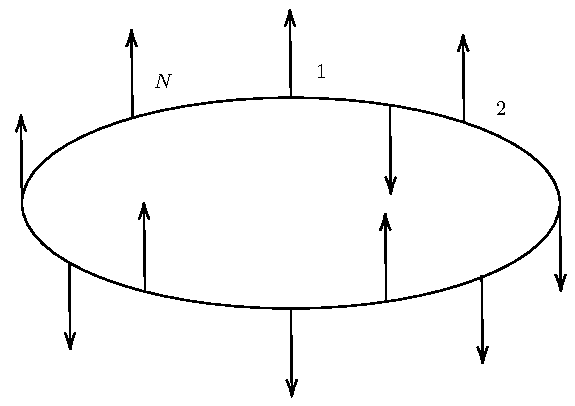
\includegraphics[width=0.5\textwidth]{../lessons/6_image/4.pdf}
\caption{\label{fig:6_4} One dimensional lattice ring.}
\end{figure}
Consider the spins sitting on a 1D lattice ring as in Figure \ref{fig:6_4}. The periodic boundary conditions are:
\begin{equation}
  S_{N+1}=S_1
\end{equation}
We have:
\begin{equation}
  -\beta \mathcal{H}_ \Omega  ( \{ S \}  ) = K \sum_{i=1}^{N} S_i S_{i+1} + h \sum_{i=1}^{N} S_i
\end{equation}
where
\begin{equation}
   K \equiv \beta J,  \quad h \equiv \beta H
\end{equation}
The \( 1-dimensional \) Ising model with this setup can be solved in several ways. Here we will use the method of the transfer matrix. This is a quite general technique that we will discuss within the Ising model.












\end{document}
